\section{Grafiskt användargränssnitt}
Beskrivning av användande av GUI:t till QuadOpt. Användarhandledningen förutsätter att du står i (\emph{/QuadOptGUI}) som skapades under installationen. En bild på hur det grafiska användargränssnittet ser ut kan ses i figur \ref{fig:gui}.


\subsection{Användning}
\begin{enumerate}
\item Öppna GUI.py på valfritt sätt. Vi rekommenderar att du gör det genom en terminal-applikation genom att skriva \emph{python3 GUI.py}.
\newline
\newline
\textbf{OBS!} Det kan hända att användargränssnittet inte startar på grund av felmeddelandet \emph{ImportError: No module named '\_tkinter'}. Då måste \emph{tkinter} installeras.
\item Skriv in ditt problem i textredigeraren som finns i GUI:t.
\item När problemet väl är inskrivet kan knappen \emph{Generate C code} användas. Denna knapp skapar filen result.c som består av problemet som skall lösas.
\item När en fil väl är genererad kan knappen \emph{Run code} användas. Denna knapp kompilerar och kör filen result.c i terminal-applikationen och presenterar optimallösningen. 
\newline
\newline
\textbf{Alternativt} kan anropet \emph{make} köras i terminalen och result.c kommer då att kompileras samt köras.
\end{enumerate}

\subsection{Kortkommandon}
Användargränsnittet stödjer ett fleralet kortkommandon. Noterbart är att ''CTRL''-knappen även gäller för Macintosh användaren och inte ''CMD''-knappen. 

\begin{itemize}
	\item \textbf{New} - CTRL+N. Öppnar en ny fil. 
	\item \textbf{Open} - CTRL+O. Öppnar utforskaren. 
	\item \textbf{Save} - CTRL+S. Sparar den öppna filen.
	\item \textbf{Save As} - CTRL+SHIFT+S. Sparar den öppna filen genom att öppna utforskaren.
	\item \textbf{Quit} - CTRL+Q. Stänger programmet.
	\item \textbf{Copy} - CTRL+C. Kopierar markerad text.
	\item \textbf{Cut} - CTRL+X. Klipper ut markerad text.
	\item \textbf{Paste} - CTRL+V. Klistrar in text.
	\item \textbf{Select All} - CTRL+A. Markerar all text.
\end{itemize}

\begin{figure}[H]
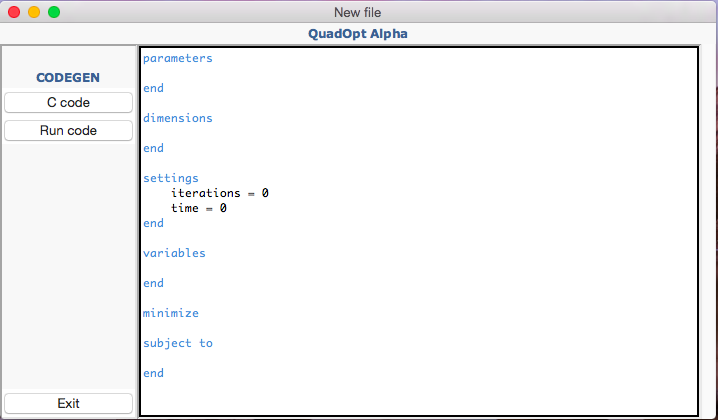
\includegraphics[scale=0.52]{bilder/macgui.png}
\caption{Det grafiska gränssnittet.}
\label{fig:gui}
\end{figure}